\documentclass[12pt]{article}
\usepackage{hyperref}
\usepackage{listings}
\usepackage[margin=1in]{geometry}
\usepackage{enumitem}
\usepackage{multicol}
\usepackage{array}
\usepackage{titlesec}
\usepackage{helvet}
\renewcommand{\familydefault}{\sfdefault}
\usepackage{amsmath}     % For math equations
\usepackage{amssymb}     % For advanced math symbols
\usepackage{amsfonts} % For math fonts
\usepackage{gvv}
\usepackage{esint}
\usepackage[utf8]{inputenc}
\usepackage{graphicx}
\usepackage{pgfplots}
\pgfplotsset{compat=1.18}
\titleformat{\section}{\bfseries\large}{\thesection.}{1em}{}
\setlength{\parindent}{0pt}
\setlength{\parskip}{6pt}
\usepackage{multirow}
\usepackage{float}
\usepackage{caption}


\begin{document}
\section*{Problem 4.12.46 :}
Find the values of $\theta$ and $p$, if the equation
\begin{align}
x\cos\theta + y\sin\theta &= p
\end{align}
is the normal form of the line
\begin{align}
\sqrt{3}x + y + 2 &= 0.
\end{align}

\section*{Solution}

We first identify the given data:

\begin{table}[H]
\centering
\begin{tabular}{|c|c|}
\hline
\textbf{Quantity} & \textbf{Value} \\
\hline
Normal vector $\vec{n}$ & $\myvec{\sqrt{3} \\ 1}$ \\
\hline
Constant $c$ & $2$ \\
\hline
\end{tabular}
\caption{}
\label{}
\end{table}

\noindent The line can be expressed as
\begin{align}
\vec{n}^T \vec{u} &= -c. \label{eq1}
\end{align}

The length of the normal is
\begin{align}
\|\vec{n}\| &= \sqrt{(\sqrt{3})^2 + 1^2} = 2. \label{eq2}
\end{align}

Thus, the unit normal becomes
\begin{align}
\hat{\vec{n}} &= \frac{\vec{n}}{\|\vec{n}\|} 
= \myvec{\tfrac{\sqrt{3}}{2} \\[4pt] \tfrac{1}{2}}. \label{eq3}
\end{align}

Dividing (3) by $\|\vec{n}\|$ gives the normal form:
\begin{align}
\hat{\vec{n}}^T \vec{u} &= \frac{-c}{\|\vec{n}\|} = -1. \label{eq4}
\end{align}

Comparing with the standard normal form
\begin{align}
x\cos\theta\, + y\sin\theta\, &= p,
\end{align}
we identify
\begin{align}
\cos\theta &= \tfrac{\sqrt{3}}{2}, \quad 
\sin\theta = \tfrac{1}{2}. \label{eq5}
\end{align}

Hence,
\begin{align}
\theta &= \tfrac{\pi}{6}, \quad p = -1. \label{eq6}
\end{align}

\noindent \textbf{Final Answer: } 
\begin{align}
\boxed{
\theta = \tfrac{\pi}{6}, \quad p = -1.
}
\end{align}

\begin{figure}[H]
    \centering
    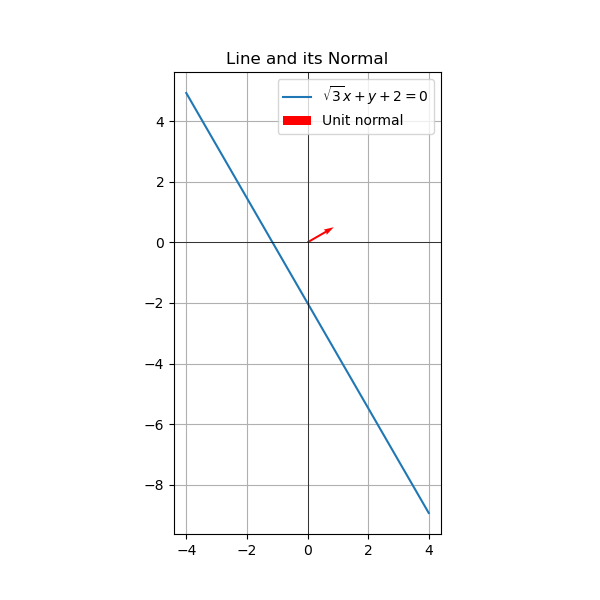
\includegraphics[width=0.9\columnwidth]{figs/normalform.png}
    \caption{}
    \label{fig:placeholder}
\end{figure}

\end{document}
